\usetikzlibrary{calc}
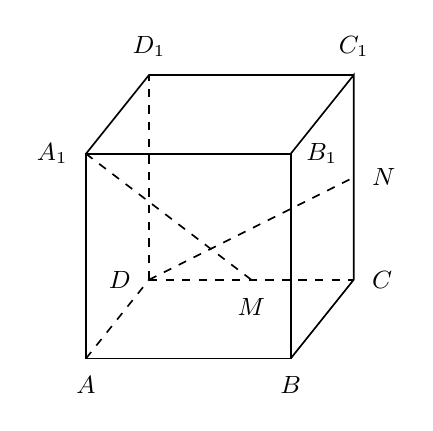
\begin{tikzpicture}[line width=.6pt, font=\small, x=1cm, y=1cm]
\coordinate (A) at (0,0);
\coordinate (B) at (2.6,0);
\coordinate (C) at (3.4,1.0);
\coordinate (D) at (0.8,1.0);
\coordinate (A1) at (0,2.6);
\coordinate (B1) at (2.6,2.6);
\coordinate (C1) at (3.4,3.6);
\coordinate (D1) at (0.8,3.6);
\coordinate (M) at (2.1,1.0);
\coordinate (N) at (3.4,2.3);
% cube solids
\draw (A)--(B)--(B1)--(A1)--cycle;
\draw (B1)--(C1)--(C)--(B);
\draw (A1)--(D1)--(C1);


% hidden
\draw[dashed] (A)--(D);
\draw[dashed] (D)--(C);
\draw[dashed] (D)--(D1);
% interior skewed lines
\draw[dashed] (A1)--(M);
\draw[dashed] (D)--(N);
% labels
\node[below=3pt] at (A) {$A$};
\node[below=3pt] at (B) {$B$};
\node[right=3pt] at (C) {$C$};
\node[left=3pt] at (D) {$D$};
\node[left=3pt] at (A1) {$A_{1}$};
\node[right=2pt] at (B1) {$B_{1}$};
\node[above=3pt] at (C1) {$C_{1}$};
\node[above=3pt] at (D1) {$D_{1}$};
\node[below=3pt] at (M) {$M$};
\node[right=3pt] at (N) {$N$};
\end{tikzpicture}
